\chapter{Plasma source description and electric characterization}
\label{ch:electric}
Plasma Coagulation Controller (PCC) developed at Consorzio RFX is a DBD cold plasma source that produces plasma at atmospheric pressure for biomedical applications. The entire design is developed to garantee the flexibility necessary to easy application on target. In this chapter the source functioning scheme is described and its features are charachterized.

\section{General source description}
Plasma is produced applying a fast high voltage pulse (from \num{2} to \SI{10}{\kilo\volt}) to a cyilindrical electrode covered by pyrex glass. The glass act as a dielectric allowing to produce plasma in DBD conditions \cite{DeMasi_2018}. The electrode is positioned along the axis of a nozzle where there is a flow of neutral gas that allows to start the discharge. The gas is a pure noble gas, sometime mixed with other gasses. It is possible to put a second electrode formed by a conducting ring around the nozzle, set to ground voltage or other voltage values, to modify the electric field if necessary.

The electrode generates an electric field that ionizes the gas producing plasma with low free charge density thanks to the glass dielectric. Plasma forms a column of glowing gas, the plasma plume, that goes out from the nozzle exit and travels in the air outside, until it reaches a certain lenght or a target, as shown in figure \ref{fig:source_scheme}. The plume is formed by cold plasma, it can be touched whitout a relevant increase of temperature on the skin or any other danger.
\begin{figure}
 \centering
 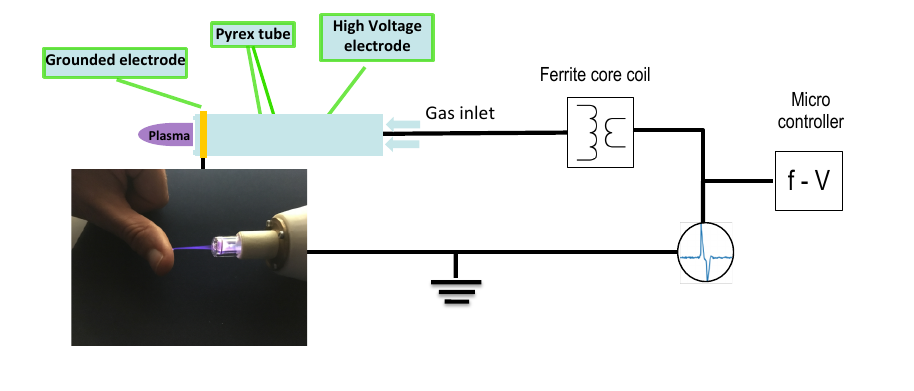
\includegraphics[width=0.9\textwidth]{Images/Electric/scheme.png}
 \caption{Scheme of the source. The micro-controller on the right sends a trigger signal to produce variable voltage on the coil mounted in the head, that produces an high voltage pulse on the electrode. The electric field ionizes the neutral gas and produces the plasma plume in the picture. The grounded ring around the nozzle is removable.}
 \label{fig:source_scheme}
\end{figure}

PCC development goes through different designs (an example of the first one is described in \cite{unipd:ceciliaDBD}). In this work are studied two different prototypes, here named \textbf{A} and \textbf{B}, with same concepts and little differences.

PCC is made of two modules: a controller box and a source head, shown in figure \ref{fig:sourcepic}.
\begin{figure}
 \centering
 \includegraphics[width=0.8\textwidth]{Images/Electric/SourcePic.png}
 \caption{Picture of PCC source, prototype \textbf{B}. The black box on the left is the \emph{Controller}, the cylinder on the right is the \emph{Head} where plasma is produced.}
 \label{fig:sourcepic}
\end{figure}

The high voltage controller is separated from the head, the first one controls the trigger for the voltage pulse, the second one is where there is plasma production.
The controller contains power cables and circuits and an Arduino Leonardo that controls pulse repetition rate and amplitude, as explained later.
The head is a cylinder \SI{30}{\centi\meter} long with diameter of \SI{8}{\centi\meter}. Inside there is a transformer made by three coils with three \emph{N87} ferrite cores of dimensions $32 \times 16 \times \SI{9}{\milli\meter}$ and induttance \SI{2.3}{\micro\henry} (\cite{N87datasheet}). The spire ratio between primary and secondary circuit of the transformer is $1/30$.
On one end of the head there is the driver circuit that receives an optical signal from the controller, that is the trigger signal for voltage pulse; on the other end there is the electrode. The driver circuit is connected to the primary circuit of the transformer, the electrode to the secondary circuit. When the controller sends the trigger signal, there is a voltage variation on primary circuit that produces the voltage pulse on the electrode.
Controller and head are connected only with power cables for driver circuit and an optical fiber that sends the trigger for the voltage pulse.

Gas is inserted trough a separated channel that goes from one end of the source to the other end near the electrode.
The nozzle at the end of the head can be selected between different materials and shapes. For this study are used a plastic nozzle that expels plasma through a cylinder with diameter of \SI{1}{\milli\meter} and a cylindrical glass nozzle that shrinks at the end, until a diameter of \SI{5}{\milli\meter}. 

Prototype \textbf{A} is the first version used during this work, prototype \textbf{B} is the latest one. Generally the second one is characterized by an higher ionization efficiency. Principal differences are:
\begin{itemize}
 \item different geometries for the coils inside the head;
 \item prototype \textbf{B} has positive voltage pulse polarity while prototype \textbf{A} has negative voltage pulse polarity;
 \item \textbf{A} presents a problem of neutral gas diffusion in the area where there are the coils due to geometry problems of the prototype. For this reason other measurements (described in following chapters) are made only with prototype \textbf{B}.
\end{itemize}

\section{Electric scheme}
In this chapter development of PCC electric scheme in discussed and its output is characterized. To produce plasma as DBD, in air, with helium or argon as ignition gasses, it is necessary to apply high voltage differance in short distances, resulting in high electric field.
It is common to produce electric fields with fast voltage pulses for various uses, including jet or DBD plasma production (\cite{Upadhyay:hvpulse}, \cite{Jarrige:plumecharacteristics}, \cite{Darny:jetplume}). The scheme that PPC uses outputs a voltage pulse with an amplitude from $\SI{1}{\kilo\volt}$ to $\SI{10}{\kilo\volt}$ and pulses repetition rates from $\SI{5}{\kilo\hertz}$ to $\SI{60}{\kilo\hertz}$.

One representation of the electric scheme is in figure \ref{fig:electricline}. As already explained, the circuit divides in two parts: the controller, with power task and voltage pulse settings, and the head, where plasma is produced.
\begin{figure}
 \centering
 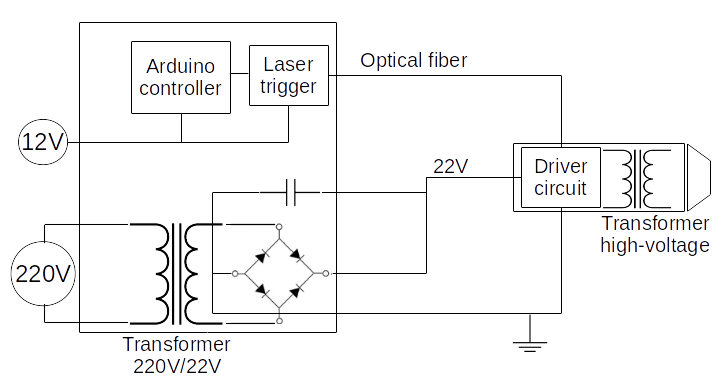
\includegraphics[width=0.9\textwidth]{Images/Electric/Linea_elettrica2.png}
 \caption{Electric scheme of the source. On the left there is the controller, on the right there is the head.}
 \label{fig:electricline}
\end{figure}

Line divides in:
\begin{itemize}
 \item \textbf{Power line} : the controller is connected to a $\SI{220}{\volt}$ AC (\SI{50}{\hertz}) power line. This signal goes in a transformer that reduces voltage value and to a diode bridge that rectifies the signal, resulting in an output of $\SI{22}{\volt}$ DC. This voltage powers the Driver Circuit on the head.
 \item \textbf{Arduino and trigger} : Arduino and a laser are connected to a power line at $\SI{12}{\volt}$. One of the Arduino analogical outputs sends a square wave (PWM) to the laser trigger, that transmits an optical signal with the same duration and pulse repetition rate of the PWM through an optical fiber. The fiber ends on a photodiode installed on the driver circuit that works as a switch to trigger the voltage pulse. With this setup pulse repetition rate and pulse amplitude are set by Arduino and the high voltage signal that circulate on the head is entirely decoupled from the controller. This setup was developed as a solution for reflection problems observed in the first PCC prototype.
 \item \textbf{Head} : on the driver circuit there are the photodiode, a capacitor and a MOSFET that works as a switch for conductive and charging phases of the circuit. When the photodiode measures the laser signal, voltage goes from power value to \num{0} and the capacitor starts charging. When the trigger signal ends, the voltage goes back to power value and the variation leads to a peak of thousends $\si{\volt}$ on the output of the secondary circuit, connected to the electrode. Pulse repetition rate, $f$, is set precisely by the Arduino, PWM duration is set giving the opening time of the MOSFET, i.e. the duration of the charging time of the capacitor. 
\end{itemize}

An example of voltage values on relevant components is presented in figure \ref{fig:signals}, obtained with a simplified scheme with Spice. Once the PWM trigger starts, voltage on the primary goes from power value to $0$, after $\SI{6}{\micro\second}$ the PWM signal ends, and the output of the secondary circuit shows a peak of $\SI{-5000}{\volt}$ and width of $\SI{1.2}{\micro\second}$. A longer PWM implies a longer charging time and an higher voltage. Ultimately, amplitude of the pulse is proportional to the width of the PWM signal and source peak output $V_p$ can be calibrated as a function of $\Delta t$ for every pulse repetition rate $f$.
It is necessary to note that when the charging phase ends, at the end of the PWM signal, there is a voltage peak also on primary circuit with amplitude of $\SI{150}{\volt}$ and several oscillations of the same amplitude on the secondary. Those could influence the output behavior if the pulse repetition rate is set too high, i.e. for values that would result in signal periods comparable to $\Delta t$.
\begin{figure}
 \centering
 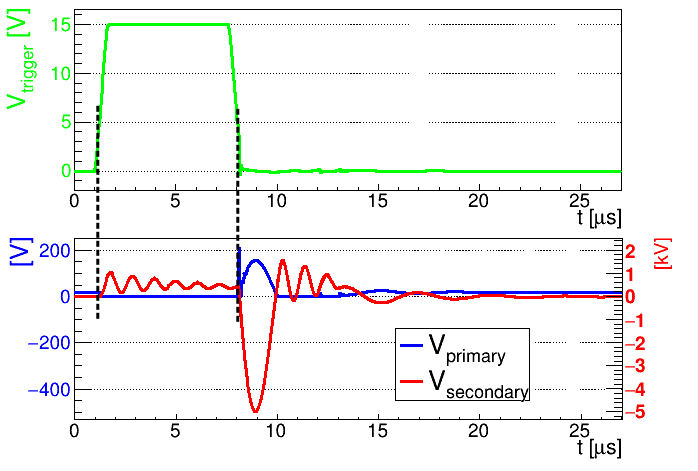
\includegraphics[width=0.8\textwidth]{Images/Electric/segnaliB2.png}
 \caption{Simulation of signals on the components of the head. Top in green there is the PWM trigger signal; bottom in blue there is the voltage of primary circuit with values in volts, in red the voltage of secondary circuit with values in kilovolts.}
 \label{fig:signals}
\end{figure}

\section{Output characterization}
The electric field generated by the electrode defines plasma production and discharge features. It is studied the dependency of plasma behavior from voltage peak value and from pulse repetition rate, $f$. In addition, medical application of plasma requires low current intensity on target, in this study it's measured current intensity flowing on a copper sheet targeted by the plasma plume at a certain distance. Ultimately the different parameters for the measures are: $\Delta t$, opening time of the MOSFET in the circuit that is proportional to voltage peak value, and $f$, pulse repetition rate. 

Voltage signals are measured with a voltage probe (\emph{hv probe}) built for high voltage measurements\emph{Tektronix P6015A}, with an attenuation factor $\times 1000$. The voltage output from secondary circuit is taken right before the connection between secondary circuit and electrode.
Current signal are measured with \emph{Tektronix CT2} current probe for current measurements. This probe have an output of $\SI{1}{\milli\volt}$ for a current of $\SI{1}{\milli\ampere}$.
An oscilloscope \emph{Yokogawa DL9040} allows to observe both signals and to store the total measured waveform.

First measurements are taken without gas flow to characterize output voltage of the circuit. After those an helium flow of $\SI{2}{\liter/\minute}$ is inserted in the head, to measure the output in presence of plasma. For both conditions the output is observed changing $\Delta t$ and for different repetition rate $f$. The average current intensity over a time period, i.e. an effective current intensity $I_{\text{eff}}$, is also observed to evaluate plasma application's effects over a longer time period.

Every lenght measure is done with a decimal caliper, that gives a measurement uncertainity of $\SI{0.1}{\milli\meter}$.

\subsection{Measurements without gas}
With a set repetition rate $f$ voltage signal is measured for different values of the opening time $\Delta t$ in the operational range.
To assure that a voltage pulse ends before another starts, this range is different for different $f$: if there are more pulses in a given time and take into consideration pulse oscillations, the range of possible $\Delta t$ is smaller for higher rates.
A typical voltage waveform is in figure \ref{fig:tensionpeak} (a). The scope of those measurements is to verify proportionality between amplitude of the peak, $V_p$, and $\Delta t$, for different $f$. Signals are analyzed with a low-pass filter where their Fourier Power Spectrum is evaluated (using ROOT C++ libraries \cite{ROOT:fft}) and the signal reconstructed without higher frequencies, to exclude noise fluctuations. The reconstructed peak is an asymmetric function in time as in figure \ref{fig:tensionpeak} (b). It is possible to fit the signal with a Landau function \cite{ROOT:landau} and obtain peak value and position.
The error on the measure is evaluated adding contributes from the low-pass filter.

\begin{comment}
\begin{figure}
 \centering
 \subfloat[Three pulses]{
    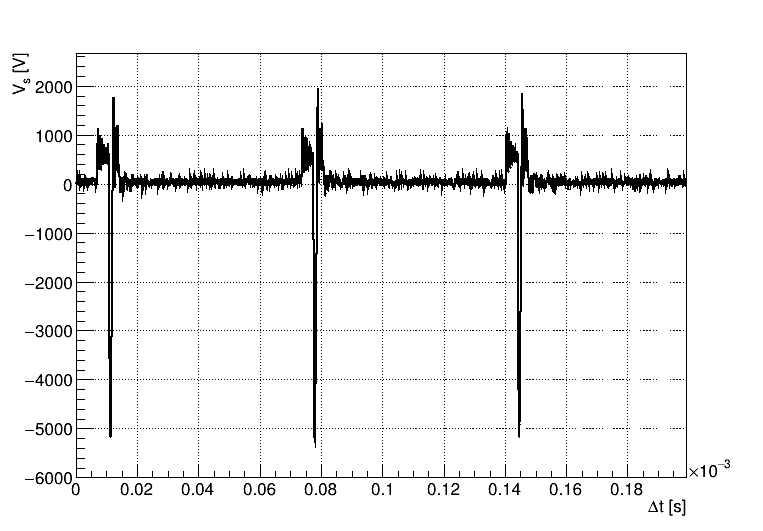
\includegraphics[width=0.40\textwidth]{Images/Electric/estrepicchi.png}
 }
 \hfill
 \subfloat[Zoom on one pulse]{
    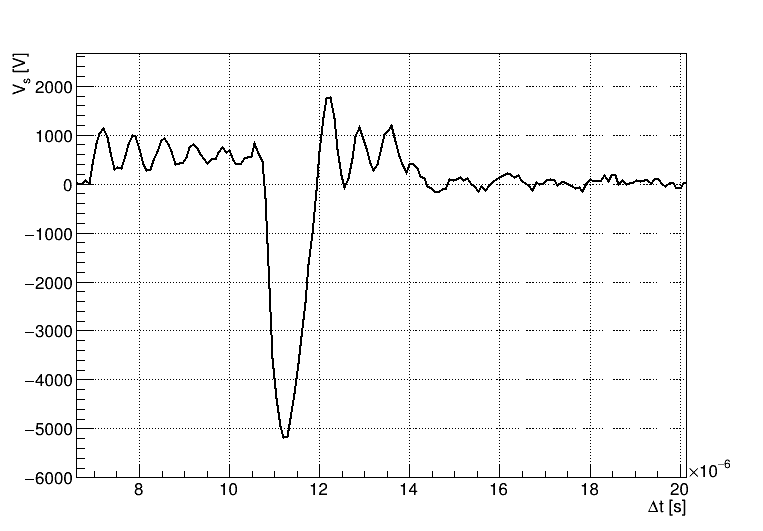
\includegraphics[width=0.40\textwidth]{Images/Electric/zoom1pk.png}
 }
 \caption{Example pulses with source B for $f = \SI{10}{\kilo\hertz}$ and $\Delta t = \SI{2}{\micro\second}$}
 \label{fig:tensionpeak}
\end{figure}

\begin{figure}
\centering
 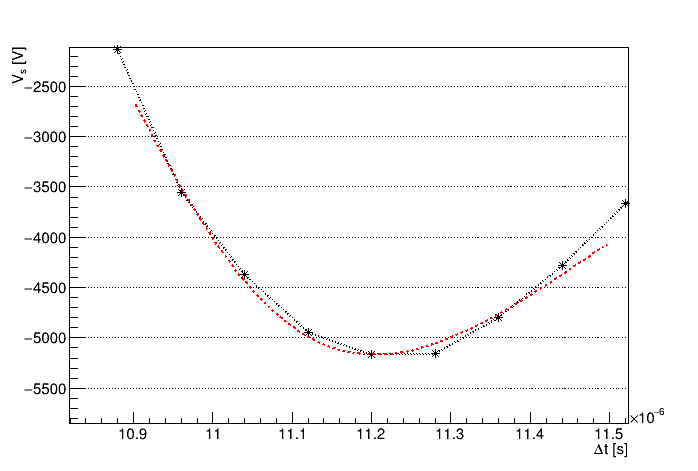
\includegraphics[width=0.6\textwidth]{Images/Electric/esfit_f10_t2.png}
 \caption{Example fit with source B for $f = \SI{10}{\kilo\hertz}$ and $\Delta t = \SI{2}{\micro\second}$}
 \label{fig:landau}
\end{figure}
\end{comment}

\begin{figure}
 \centering
 \subfloat[Voltage peak example.]{
    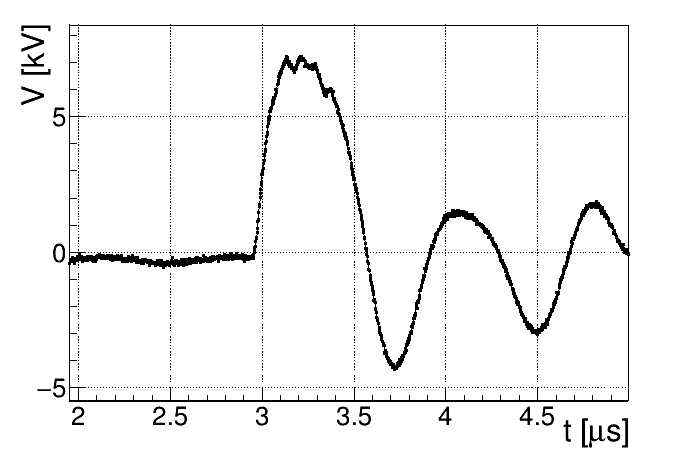
\includegraphics[width=0.48\textwidth]{Images/Electric/espicco_pos.png}
 }
 \hfill
 \subfloat[Zoom on peak fit.]{
    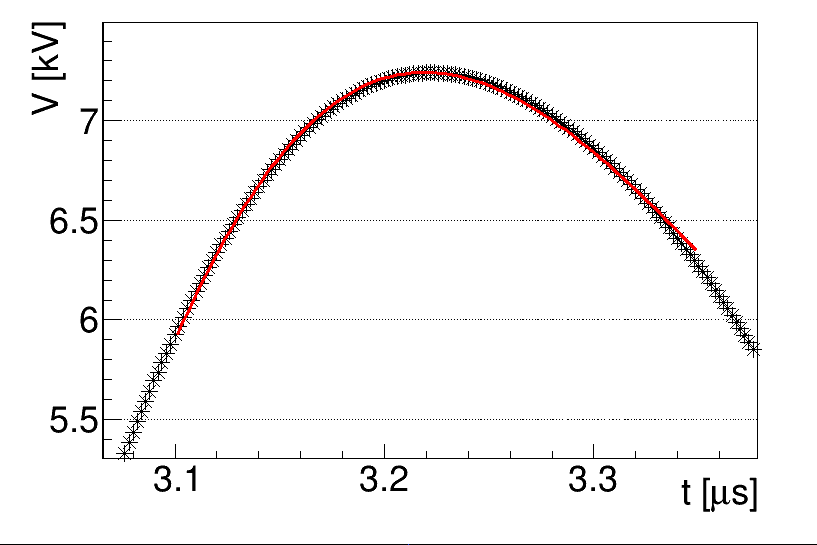
\includegraphics[width=0.48\textwidth]{Images/Electric/piccopos_fit.png}
 }
 \caption{(a) Example of voltage measurements with prototype \textbf{B} for $f = \SI{5}{\kilo\hertz}$ and $\Delta t = \SI{4}{\micro\second}$ ; (b) reconstructed signal after low pass filter and fit of the peak.}
 \label{fig:tensionpeak}
\end{figure}

Results are shown in figure \ref{fig:nogas} for prototype \textbf{A} and \textbf{B}.
For \textbf{A} there is a linear behavior for $4 \le \Delta t \le \SI{16}{\micro\second}$, with peak values from $\num{2.02(1)}$ to $\SI{9.25(5)}{\kilo\volt}$; for larger $\Delta t$ the relation is not linear. The upper limit on $\Delta t$ is given by the need of a minimum time interval between two pulses.
Also for \textbf{B} there is a linear behavior, but with higher values: for $1 \le \Delta t \le \SI{8}{\micro\second}$ voltage peak goes from $\num{3.66(6)}$ to $\SI{11.76(22)}{\kilo\volt}$. With this source the upper limit for $\Delta t$ is chosen considering the maximum voltage value sustainable by the dielectric. To avoid the risk of dielectric breakdown the maximum opening time for prototype \textbf{B} is set at $\Delta t = \SI{8}{\micro\second}$.

Voltage output doesn't show significative differances changing repetition rate. To confirm this observation measures are interpolated with a linear function in the range $0-\SI{16}{\micro\second}$ for \textbf{A} and range $0-\SI{8}{\micro\second}$ for \textbf{B}. Parameters resulting from the fit are compared as in figure \ref{fig:linnogas}. Values are displaced with random distances from the mean value, so it can be concluded that the behavior is not defined by the repetition rate.
\begin{figure}
 \centering
 \subfloat[Source A]{
    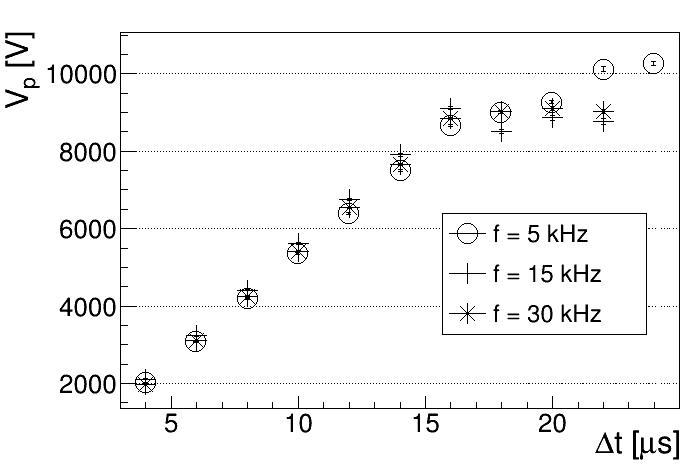
\includegraphics[width=0.48\textwidth]{Images/Electric/Vpp_nogas_A2.png}
 }
 \hfill
 \subfloat[Source B]{
    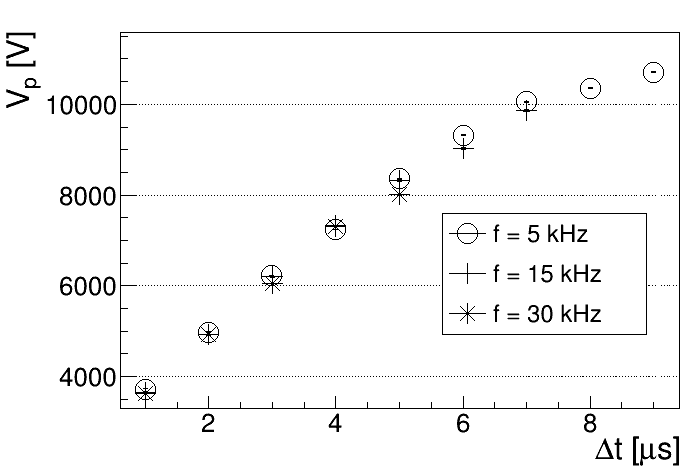
\includegraphics[width=0.48\textwidth]{Images/Electric/Vpp_nogas_B2.png}
 }
 \caption{Absolute voltage peak values of secondary circuit output in function of $\Delta t$ at different $f$, for both prototypes. Voltage peaks show linear behavior for $V_p \le \SI{10}{\kilo\volt}$.}
 \label{fig:nogas}
\end{figure}

\begin{figure}
 \centering
 \subfloat[Source A]{
    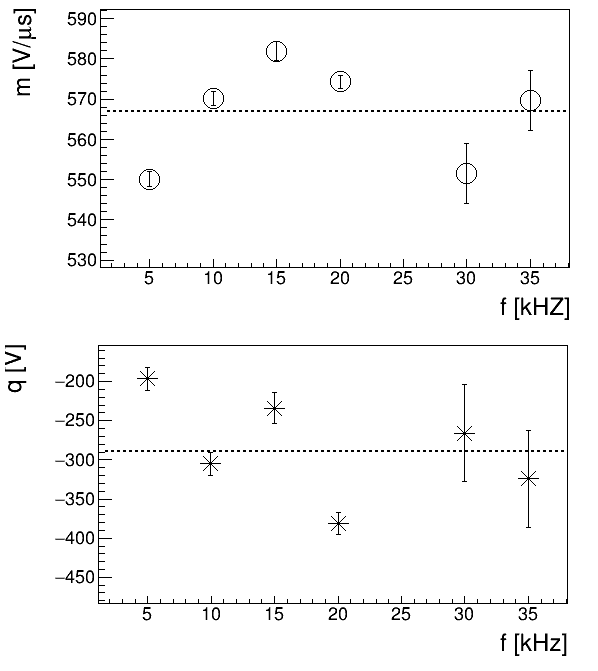
\includegraphics[width=0.48\textwidth]{Images/Electric/mq_nogas_A2.png}
 }
 \hfill
 \subfloat[Source B]{
    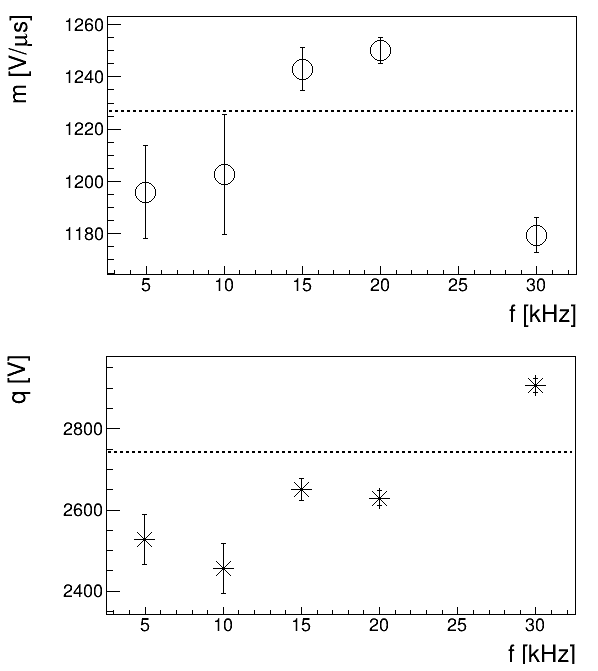
\includegraphics[width=0.48\textwidth]{Images/Electric/mq_nogas_B2.png}
 }
 \caption{Resulting parameters from the linear fit of voltage values as a function of opening time without plasma, for different repetition rates, for both prototypes. Voltage peaks are interpolated with a linear function $V_{peak} = m \Delta t + q$, in figure there are slopes $m$ on top and intercepts $q$ on bottom. Dashed line is the average value of the parameter. There isn't a specific behavior in parameters, is possible to conclude that output voltage does not depend on pulse repetition rate.}
 \label{fig:linnogas}
\end{figure}


\subsection{Measurements with gas}
Helium gas with a flow of \SI{2}{\liter/\minute} is introduced at the end of the head, near the electrode, to produce plasma in DBD conditions. Measurements are repeated as before to study how voltage value changes with plasma introduction.
A conductive target is placed in front of the source to measure the intensity of current carried by plasma. To assure safety of plasma application large current intensities and the possibility of arc formation needs to be avoided. Studies of conditions for DBD discharges and arc transitions (\cite{kogelschatz:jpa-00255561}, \cite{TOMAI2006409}, \cite{PhysRev.34.876}) suggests that for fast pulses it's safe to have current intensity $< \SI{10}{\milli\ampere}$.

Current intensity is measured with a copper sheet of dimensions $\SI{10}{\milli\meter} \times \SI{10}{\milli\meter} \times \SI{1}{\milli\meter}$. The plasma plume impacts on the sheet that is connected to the current robe that converts the signal in a voltage measurements that the oscilloscope can measure. Due to low current intensities it is necessary to pay attention to cables shielding, decreasing noise.
The relation between current intensity and target distance is studied in \cite{unipd:ceciliaDBD}. In this work the distance between target and electrode is choosen around typical values for treatments: $\SI{10}{\milli\meter}$ for prototype \textbf{A} and $\SI{15}{\milli\meter}$ for prototype \textbf{B}.

In figure \ref{fig:tens_curr} is presented a measure for $\Delta t = \SI{8}{\micro\second}$ and $f =\SI{5}{\kilo\hertz}$ with prototype \textbf{B}. For both sources there is a current peak in correspondence of voltage pulse, that increases with voltage.
\begin{figure}
\centering
 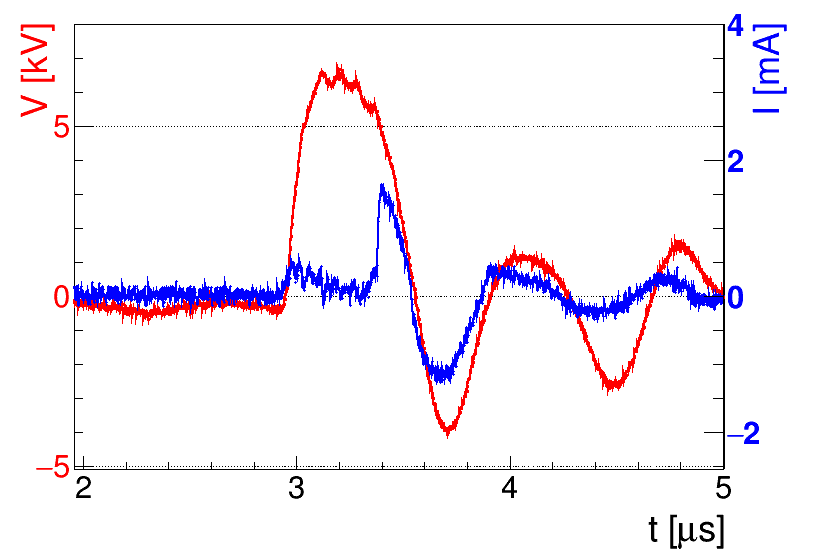
\includegraphics[width=0.6\textwidth]{Images/Electric/espiccopos_corrente.png}
 \caption{Voltage output (red) and current measurements (blue) for a discharge  with prototype \textbf{B}, $f = \SI{5}{\kilo\hertz}$ and $\Delta t = \SI{3}{\micro\second}$}
 \label{fig:tens_curr}
\end{figure}

Data analysis is the same described before, for both voltage and current values. Results are shown in figures \ref{fig:Vpp_gas} and \ref{fig:I_gas}, measurements where the current peak is not distinguishable from noise are excluded from plots.
\begin{figure}
 \centering
 \subfloat[Source A]{
    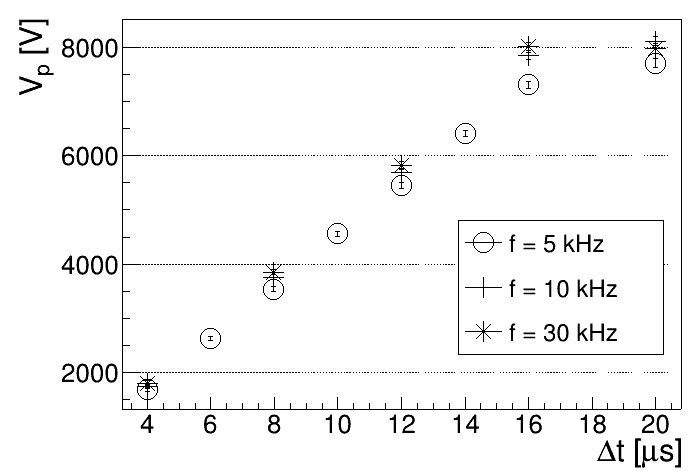
\includegraphics[width=0.48\textwidth]{Images/Electric/Vpp_gas_A2.png}
 }
 \hfill
 \subfloat[Source B]{
    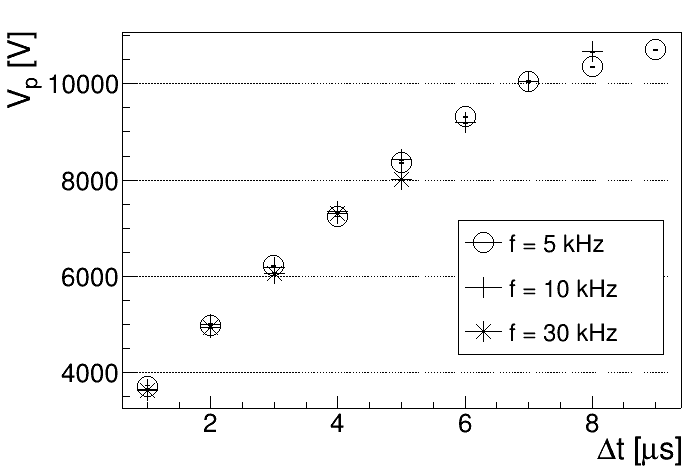
\includegraphics[width=0.48\textwidth]{Images/Electric/Vpp_gas_B2.png}
 }
 \caption{Absolute voltage peak values of secondary circuit as a function of $\Delta t$ at different $f$, with an helium flux of $\SI{2}{\liter/\minute}$, for both sources.}
 \label{fig:Vpp_gas}
\end{figure}

\begin{figure}
 \centering
 \subfloat[Source A]{
    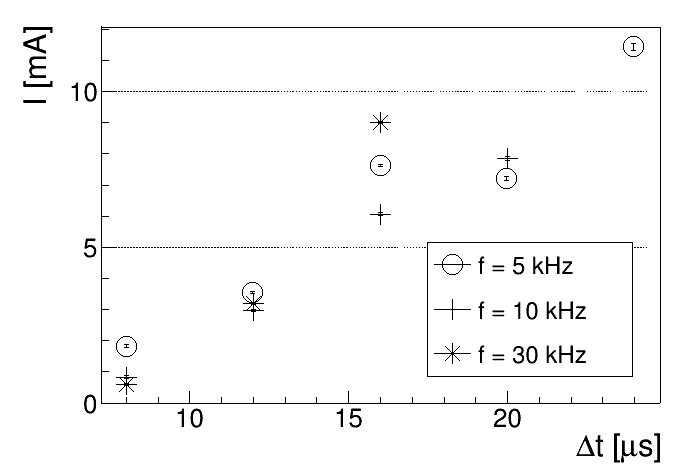
\includegraphics[width=0.48\textwidth]{Images/Electric/I_gas_A2.png}
 }
 \hfill
 \subfloat[Source B]{
    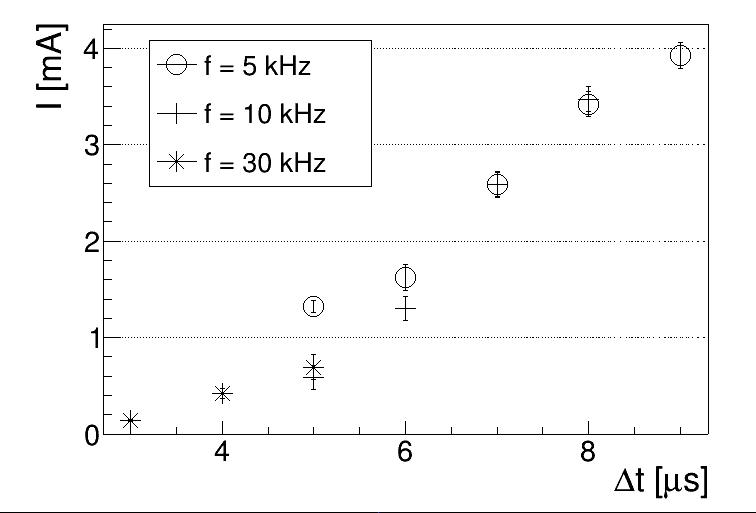
\includegraphics[width=0.48\textwidth]{Images/Electric/I_gas_B2.png}
 }
 \caption{Absolute current peak values measured with helium flux of $\SI{2}{\liter/\minute}$, on a copper target, as a function of $\Delta t$ at different $f$, for both sources.}
 \label{fig:I_gas}
\end{figure}

Voltage peaks are lower then values without gas. It is an expected behavior if the plume is considered as an additional resistive load at the end of the circuit \cite{lieberman1994principles}. Also for this measurements there is a linear dependency between voltage and $\Delta t$ for $V_{p} \le \SI{10}{\kilo\volt}$. Linear fit parameters are again compared for different $f$. Current intensities increase as voltage and are higher for prototype \textbf{A}, as expected given different distances electrode-target. Analysis of linearity also for those measures can show if there is a different behavior changing pulse repetition rate.
Figures \ref{fig:lingas_Vpp} and \ref{fig:lingas_I} shows results of the linearity study for different pulse rates.

For voltage fit parameters are scattered around their average value for both sources, confirming the hypotesis that voltage growth is independent from pulse repetition rates. For prototype \textbf{A} the voltage average increase is $m_{V} = \SI{0.366(1)}{\kilo\volt/\micro\second}$, for prototype \textbf{B} is $m_{V} = \SI{1.145(8)}{\kilo\volt/\micro\second}$, higher, as explained before.

Current values shows a different behavior: in prototype \textbf{A} there are increasing parameters with increasing repetition rates, in prototype \textbf{B} data are more scattered and it is not possible to extrapolate a behavior. Despite this behavior the slope is in the same range of values for both prototypes, with a maximum for \textbf{A} of $m_{I} = \SI{1.10(1)}{\milli\ampere/\micro\second}$ and for \textbf{B} of $m_{I} = \SI{1.04(17)}{\milli\ampere/\micro\second}$.

The parameter trend in prototype \textbf{A} could suggest a variation of reaction parameters happening inside the plasma. If with higher repetition rate there are more ionization reactions, there would be higher charge densities and higher measured current intensity. Due to low signal to noise ratio in measures for prototype \textbf{B}, it is not possible to esclude a relation between current slope and repetition rate for this source, however it is established a maximum limit value to take into consideration when using the device.
\begin{figure}
 \centering
 \subfloat[Source A]{
    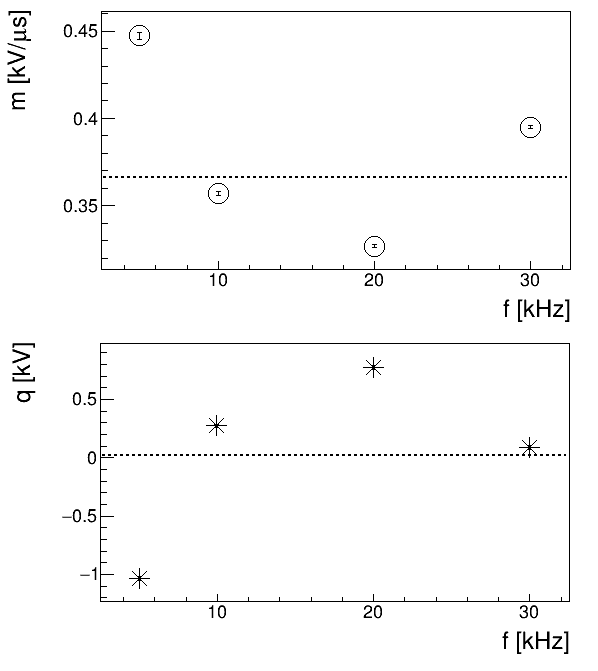
\includegraphics[width=0.48\textwidth]{Images/Electric/mq_V_gas_A2.png}
 }
 \hfill
 \subfloat[Source B]{
    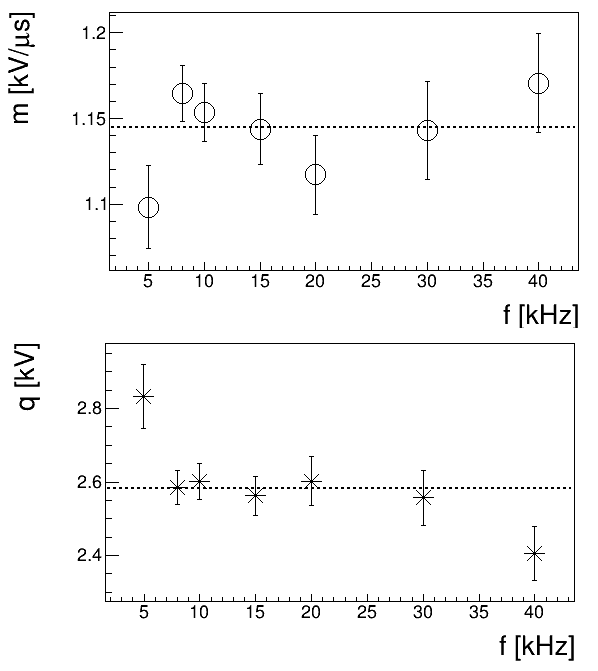
\includegraphics[width=0.48\textwidth]{Images/Electric/mq_V_gas_B2.png}
 }
 \caption{Resulting parameters from the linear fit of voltage values as a function of opening time in presence of plasma, for different repetition rates, for both prototypes. Voltage peaks are interpolated with a linear function $V_{peak} = m \Delta t + q$, in figure there are slopes $m$ on top and intercepts $q$ on bottom. Dashed line is the average value of the parameter. Also with plasma there is not a  specific behavior in parameters. It is possible to conclude that output voltage does not depend on pulse repetition rate.}
 \label{fig:lingas_Vpp}
\end{figure}


\begin{figure}
 \centering
 \subfloat[Source A]{
    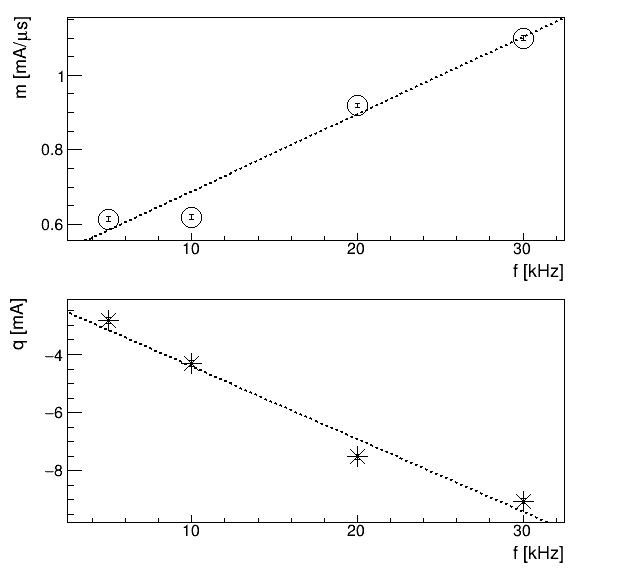
\includegraphics[width=0.48\textwidth]{Images/Electric/mq_I_gas_A2.png}
 }
 \hfill
 \subfloat[Source B]{
    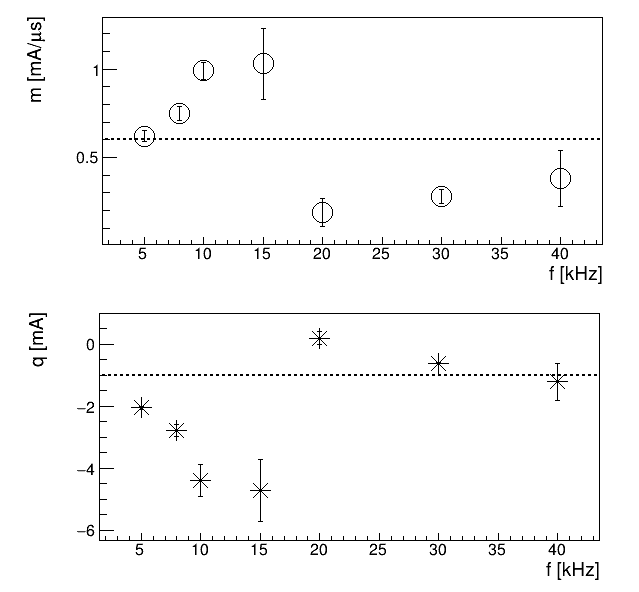
\includegraphics[width=0.48\textwidth]{Images/Electric/mq_I_gas_B2.png}
 }
 \caption{Resulting parameters from the linear fit of current values as a function of opening time, for different repetition rates, for both prototypes. Current peaks are interpolated with a linear function $I_{peak} = m \Delta t + q$, in figure there are slopes $m$ on top and intercepts $q$ on bottom. Dashed line is the average value of the parameter. For prototype \textbf{A} there is a linear dependency from $f$, in dashes in the figure. For prototype \textbf{B} it is not possible to extrapolate a behaviour.}
 \label{fig:lingas_I}
\end{figure}

\paragraph{Time intervals}
From voltage and current waveforms it is possible to extrapolate informations on time width of those signals. They can be defined as the FWHM of measured peaks, evaluated as the time when we measure half of tension or current maximum value. As the characterization of the sources shows an almost equal behavior, this study is made only for prototype \textbf{B}, that is the only one used in the following chapters. Results are shown in figure \ref{fig:times}.
For every repetition rate there is a quadratic behavior of voltage widths with a minimum for a $\Delta t = \SI{5}{\micro\second}$. It is possible to give an estimation of pulse width with a mean value between this minimum and maximum values obtained for $\Delta t = \SI{1}{\micro\second}$, it is $T_{V} = \SI{963(15)}{\nano\second}$. For currents, widths have great uncertainity where the peak is low, but it is possible to evaluate a mean value for $\Delta t \ge \SI{6}{\micro\second}$, and it is $T_{I} = \SI{968(28)}{\nano\second}$.
Values from the two measurements are compatible and they are a good estimation of pulse time duration.

\begin{figure}
 \centering
 \subfloat[Voltage]{
    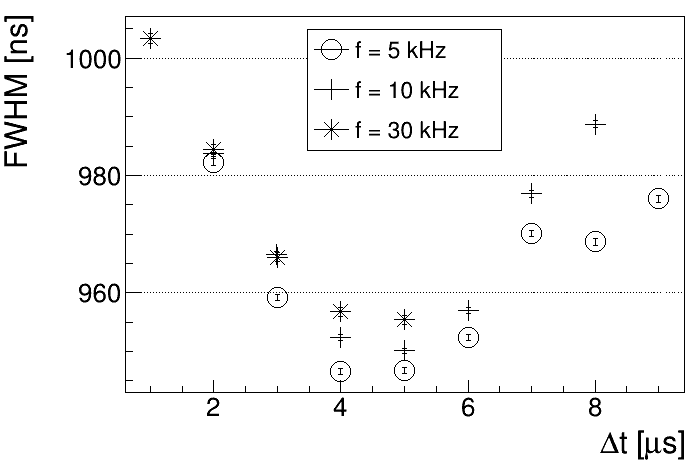
\includegraphics[width=0.48\textwidth]{Images/Electric/tempi_V2.png}
 }
 \hfill
 \subfloat[Current]{
    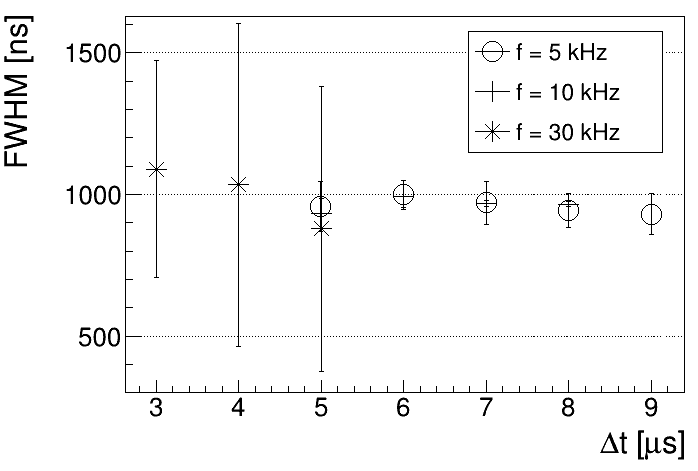
\includegraphics[width=0.48\textwidth]{Images/Electric/tempi_I2.png}
 }
 \caption{FWHM of voltage and current pulses varying opening time, for different pulse repetition rates.}
 \label{fig:times}
\end{figure}


\subsection{Effective current}
Current effects in applications on biological tissues have to take into consideration current intensity in a time interval tipically larger then the pulse widths used in our sources (\cite{doi:10.1002/ppap.200731208}, \cite{unipd:ceciliaDBD}). It's possible to estimate an effective current that is more appropriate to take into consideration when evaluating damage due to currents, as a mean of current intensity in a defined time interval calculated with equation \ref{eq:ieff}, taking $t_2-t_1 = \SI{1}{\milli\second}$. The effective current takes into consideration that current values are very small for all the time between two pulses.
\begin{equation}
 \centering
 I_{\text{eff}} = \sqrt{\frac{1}{(t_2-t_1)}\int_{t_1}^{t_2} I^2 \,dt}
 \label{eq:ieff}
\end{equation}

Figure \ref{fig:ieff} shows effective currents measured for both sources. Values are significantly smaller then maximum peak values, expecially for prototype \textbf{B} where oscillations after the main peak are smaller. The maximum value for the two prototypes is given by $I_{\text{eff} A} = \SI{2.47(7)}{\milli\ampere}$ and $I_{\text{eff} B} = \SI{0.23(1)}{\milli\ampere}$.

\begin{figure}
 \centering
 \subfloat[Source A]{
    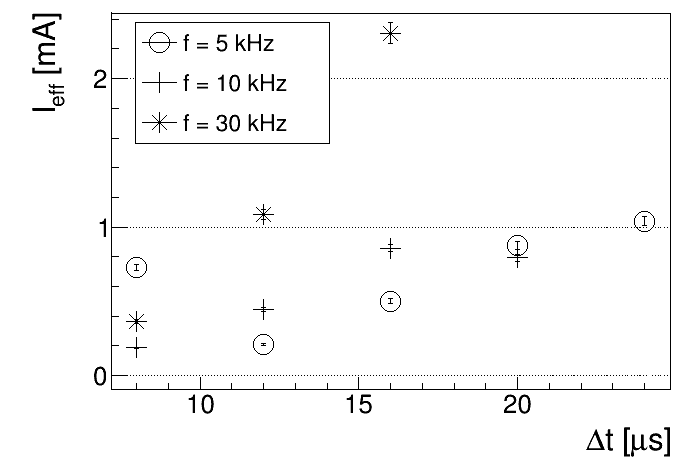
\includegraphics[width=0.48\textwidth]{Images/Electric/Ieff_A2.png}
 }
 \hfill
 \subfloat[Source B]{
    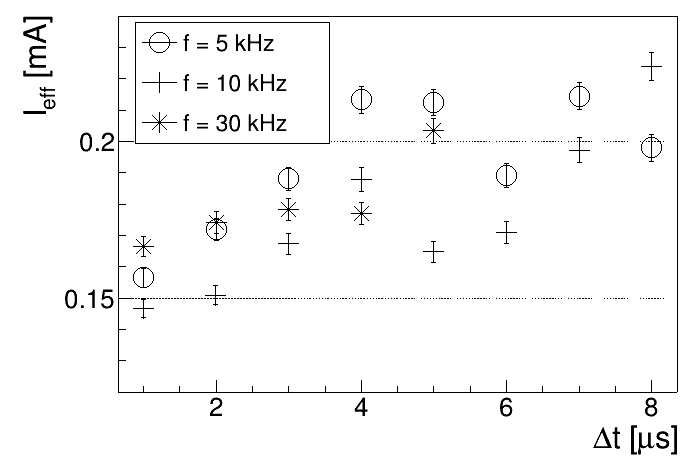
\includegraphics[width=0.48\textwidth]{Images/Electric/Ieff_B2.png}
 }
 \caption{Effective current values measured for a time interval of $\SI{1}{\milli\second}$ as a function of $\Delta t$, for different repetition rates, for both sources.}
 \label{fig:ieff}
\end{figure}


\subsection{Plasma impedance estimate}
From voltage and current measuraments can be extrapolated plasma's electric behavior. In this subsection plasma impedance is estimated with measurements from prototype \textbf{B}. Voltage output from head's transformer can be modelized as a damped sine wave around the peak, as in equation \ref{eq:dmpsin}, where $V_{\text{pulse}}$ is the amplitude of the undamped pulse, $\tau$ is the characteristic damping time and $f_{V_{s}}$ is the explicit parametrization of the frequency of the single pulse that we observe on measurements.
\begin{equation}
 V_{S} = V_{0} + V_{\text{pulse}} \sin{(2 \pi f_{V_{s}} t)} e^{-t/\tau}
 \label{eq:dmpsin}
\end{equation}

It's possible to study how plasma impedance changes for different frequency pulse $f_{V_{s}}$ to understand its electric behavior. Frequency pulse is different for each opening time of the circuit, $\Delta t$, but it is constant when changing pulse repetition rate, as explained before analyzing voltage outputs. In figure \ref{fig:fitexp} there is an example of a peak interpolated with the function in formula \ref{eq:dmpsin} %and it's power spectrum that shows the peak at a value corresponding to $f_{V_s}$ for that specific $\Delta t$.
while in figure \ref{fig:parexp} there are the resulting fit parameters for different $\Delta t$.
\begin{figure}
 \centering
 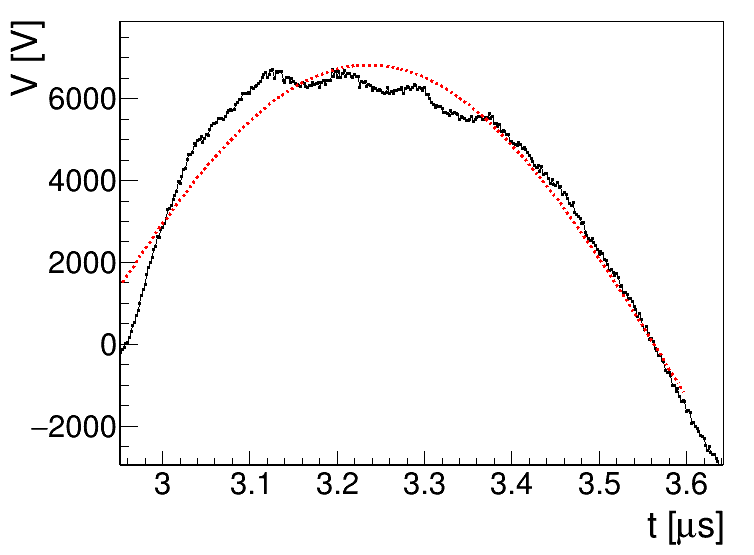
\includegraphics[width=0.5\textwidth]{Images/Electric/VFitexp_f8_t5_2.png}
 \caption{Example of a fit of voltage measurements with function \ref{eq:dmpsin}.}
 \label{fig:fitexp}
\end{figure}

\begin{comment}
\begin{figure}
 \centering
 \subfloat[Dumped sin fit]{
    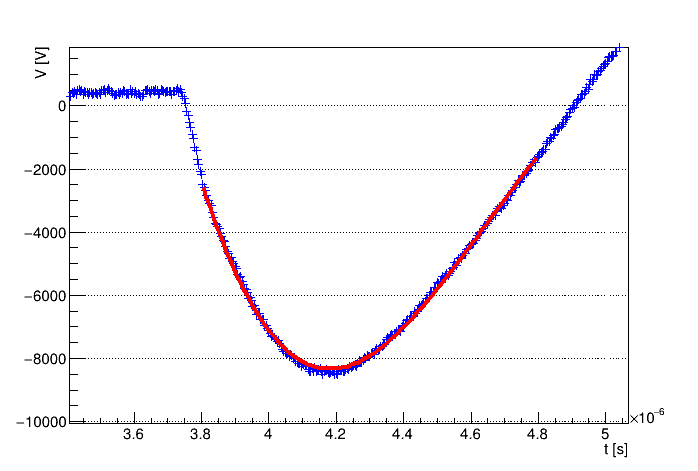
\includegraphics[width=0.4\textwidth]{Images/Electric/VFitexp_f8_t5.png}
 }
 \subfloat[Power spectrum]{
    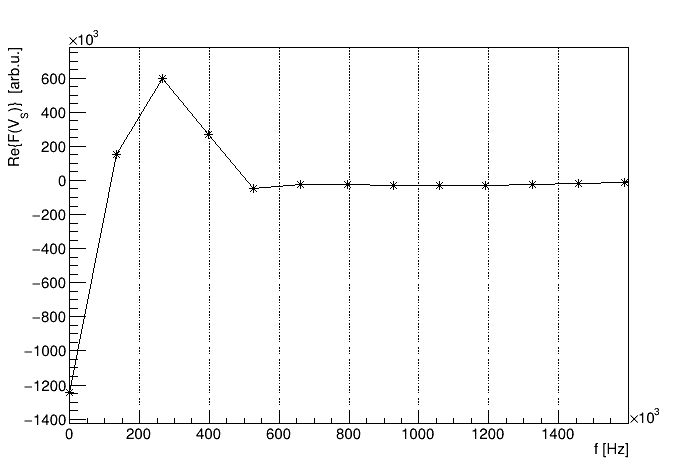
\includegraphics[width=0.4\textwidth]{Images/Electric/Trasf_f8_t5_clean.png}
 }
 \caption{On the left example fit of a tension peak, $f = \SI{8}{\kilo\hertz}$ $\Delta t = \SI{5}{\micro\second}$ with function \ref{eq:dmpsin}; on the right the fourier transform of the measure in the interval [$3-\SI{6}{\micro\second}$] that shows the frequency peak $f_{V_s}$}
 \label{fig:fitexp}
\end{figure}
\end{comment}

\begin{figure}
 \centering
 \subfloat[$V_{\text{pulse}}$]{
    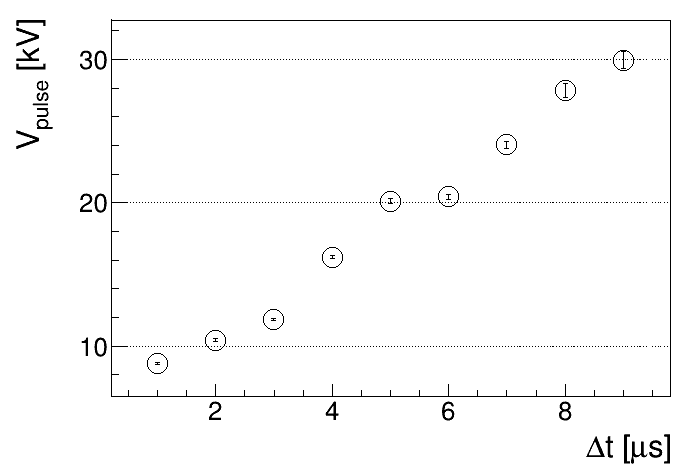
\includegraphics[width=0.48\textwidth]{Images/Electric/ParfitExp_Vp.png}
 }
 
 \subfloat[$\tau$]{
    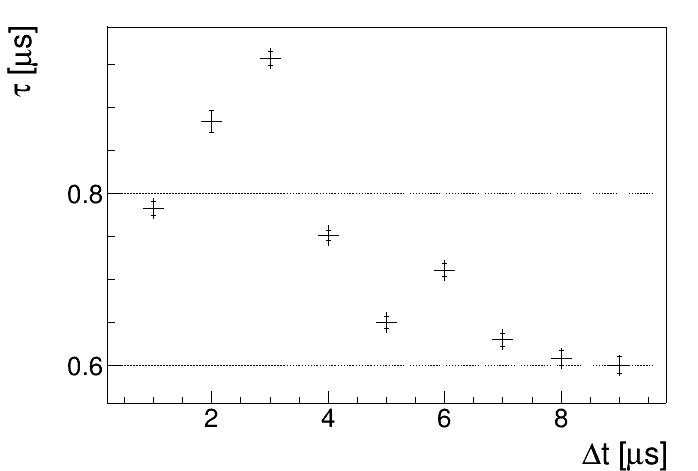
\includegraphics[width=0.48\textwidth]{Images/Electric/ParfitExp_T.png}
 }
 \hfill
 \subfloat[$f_{V_s}$]{
    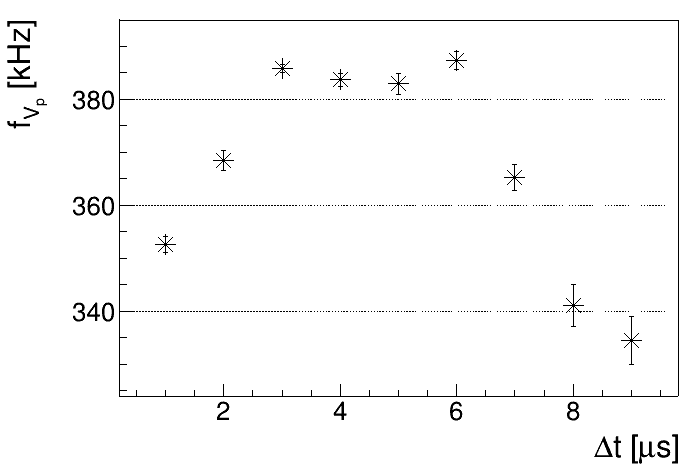
\includegraphics[width=0.48\textwidth]{Images/Electric/ParfitExp_f.png}
 }
 \caption{Resulting parameters from the interpolation of measurements with a dumped sin, as in equation \ref{eq:dmpsin}, for pulses with $f=\SI{8}{\kilo\hertz}$ and different $\Delta t$.}
 \label{fig:parexp}
\end{figure}

With higher opening times $ V_{\text{pulse}}$ is higher as expected, while $f_{V_{s}}$ and $\tau$ have their own behaviors that depends from $V_s$.
To estimate plasma's impedance it's useful to observe that voltage peak is quite large in time: it varies of less then $3\%$ of peak's value in an interval of $\SI{150}{\nano\second}$ around it. As voltage and current peak times differ always by a time interval $|t_{V_p} - t_{I_p}| \leq \SI{150}{\nano\second}$, it is possible to assume $V_{t_{I_p}} \simeq V(t_{V_p})$, i.e. that voltage during the current peak maximum is equal to voltage peak value. With this approximation, voltage peak values can be studied as a function of current peak value, as in figure \ref{fig:viplot}. An estimation of average plasma resistance is the slope resulting from a linear fit or it is possible to estimate the resistance as $R = \frac{V_{p}}{I_{p}}$ for a particular $\Delta t$ . Results are shown in figure \ref{fig:zest}, changing opening times and changing frequency of single pulse $f_{V_{s}}$.

\begin{figure}
 \centering
 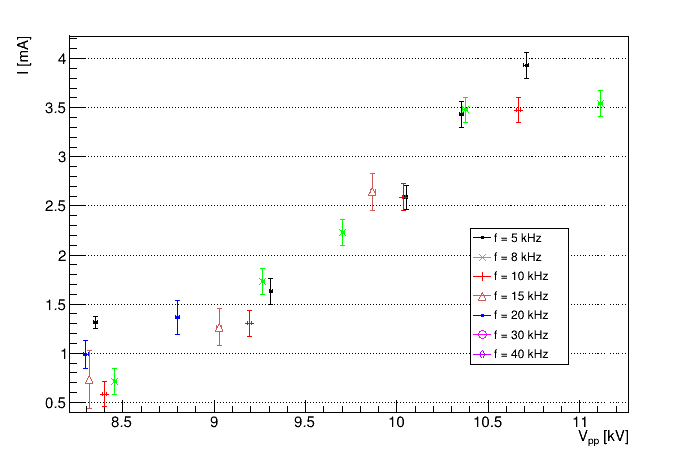
\includegraphics[width=0.65\textwidth]{Images/Electric/VI_B.png}
 \caption{Voltage peak values against current peak values for different $f$.}
 \label{fig:viplot}
\end{figure}

\begin{figure}
 \centering
 \subfloat[$R$ as a function of $\Delta t$]{
    \includegraphics[width=0.48\textwidth]{Images/Electric/Rdt.png}
 }
 \subfloat[$R$ as a function of $f_{V_s}$]{
    \includegraphics[width=0.48\textwidth]{Images/Electric/RfVs.png}
 }
 \caption{Plasma resistance for different opening times (a) corresponding to different frequencies fit parameter (b).}
 \label{fig:zest}
\end{figure}

From the graphs it's possible to extrapolate that plasma resistance goes from $\SI{2.98(11)}{\mega\ohm}$ to $\SI{11.82(219)}{\mega\ohm}$, with near constant values in the range of opening times $7-\SI{9}{\micro\second}$.
From a deeper analysis and specific measures it could be possible to expand the analysis here presented and estimate plasma's electrical capacitance or induttance.




\begin{comment}

\subsection{Corrente efficace}
Durante l'applicazione del plasma su tessuti vivi bisogna considerare il tempo di reazione effettivo del bersaglio, l'impulso di corrente alle frequenze di lavoro della sorgente presenta un periodo inferiore rispetto questi tempi. Per valutare gli effetti del trattamento viene calcolato il valore della corrente efficace che fluisce sulla piastra bersaglio in un tempo di \SI{1}{\milli\second}, dell'ordine di grandezza dei tempi di risposta da considerare (vedi articolo?), utilizzando la formula in \ref{eq:ieff}.
\begin{equation}
 \centering
 I_{\text{eff}} = \frac{1}{(t_2-t_1)}\sqrt{\int_{t_1}^{t_2} I^2 \,dt}
 \label{eq:ieff}
\end{equation}

In Figura \ref{fig:correff} vengono presentati i valori della corrente efficace in maniera simile a quanto fatto per le misure di corrente precedentemente.
A parità di tempo di apertura del circuito, una maggiore frequenza implica che nel tempo scelto di \SI{1}{\milli\second} vi sarà un numero di periodi maggiore, aumentando la corrente efficace nel circuito. In figura si vede come mediamente la corrente efficace sia più grande a frequenze maggiori, ma assume sempre valori inferiori ai \SI{3}{\milli\ampere}.

\begin{figure}
\centering
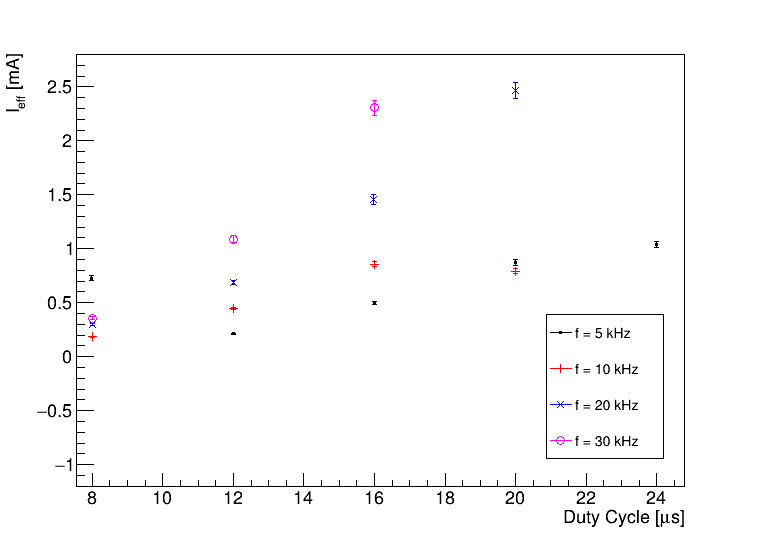
\includegraphics[width=.7\textwidth]{Immagini/ieff.png}
\caption{Corrente efficace calcolata al variare del tempo di apertura del circuito e per diverse frequenze.}
\label{fig:correff}
\end{figure}

\end{comment}


\begin{comment}
La sorgente di plasma funziona tramite l'applicazione di un'alta differenza di potenziale tra gli elettrodi separati da materiale dielettrico, come descritti nel capitolo \ref{ch:sorgente}. La tensione in ingresso nel circuito  della testa della sorgente vengono amplificati fino a tensioni di alcuni \si{\kilo\volt}. Dall'arduino di controllo è possibile regolare il tempo di apertura del circuito in un range di [$2$-$20$] \si{\micro\second} e la frequenza di lavoro in un range di [$2$-$60$] \si{\kilo\hertz}. I parametri importanti per caratterizzare il funzionamento della sorgente saranno quindi tensione e corrente all'uscita del circuito secondario del trasformatore, al variare dei parametri di funzionamento. Utilizzando una lastra metallica posta a potenziale, è possibile misurare la corrente in un dato range temporale. È inoltre possibile stimare la corrente efficace che attraversa il bersaglio, importante nel valutare gli effetti dell'applicazione del plasma.

\section{Setup delle misure di tensione e corrente}
Si vogliono effettuare misure di tensione della sorgente sia senza immissione di elio, senza formazione della plume di plasma, sia nelle condizioni di funzionamento tipiche, con flusso di elio di $\SI{2}{\liter/\minute}$.
Le tensioni vengono misurate tramite una sonda \emph{...} con attenuazione $\times1000$, le correnti tramite una sonda \emph{Tektronix CT2} che per una corrente di \SI{1}{\milli\ampere} restituisce un segnale di \SI{1}{\milli\volt}. I dati vengono letti su un oscilloscopio \emph{Yokogawa DL9040}, che permette il salvataggio dell'intera forma d'onda misurata nei diversi canali. 
Viene effettuata la caratterizzazione elettrica di entrambi i prototipi di sorgente, per i quali il circuito utilizzato è lo stesso, quindi non si aspettano variazioni significative.
\end{comment}



\begin{comment}

\subsection{Misure senza elio}
La sonda ad alta tensione viene collegata all'uscita del circuito secondario, mentre una sonda con attenuazione $\times10$ viene utilizzata per controllare il segnale in ingresso.
La sorgente viene azionata variando la frequenza ($f$) e duty cycle ($\Delta t$). Scelta la frequenza di lavoro, viene variata la duty cycle in un range utile, considerando il tempo necessario al terminare delle oscillazioni del segnale prima dell'arrivo di una nuova onda quadra (per frequenze maggiori si potrà arrivare a duty cycle minori).
Si ottengono curve come in figura \ref{fig:tensione_es}. La risoluzione della misura viene variata in modo da avere l'errore di misura minore possibile.

\begin{figure}
\centering
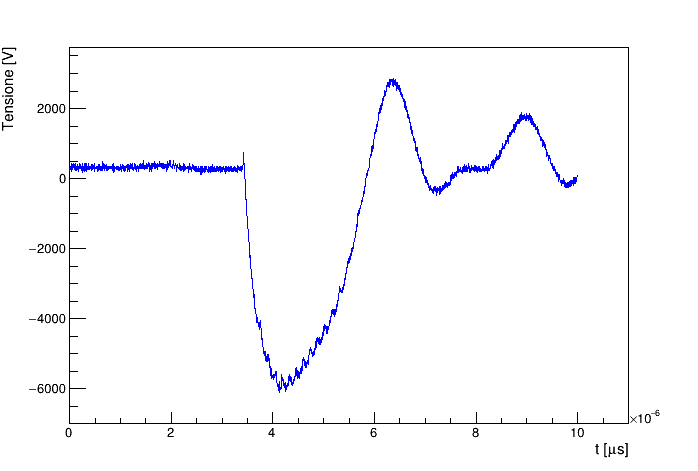
\includegraphics[width=.7\textwidth]{Immagini/tensione_es_2.png}
\caption{Esempio di misura di tensione, $f = \SI{5}{\kilo\hertz}$ e $\Delta t = \SI{16}{\micro\second}$, prototipo 1.}
\label{fig:tensione_es}
\end{figure}



\section{Presentazione misure ed analisi}
Sia per le misure di tensione che per le misure di corrente si trova un picco negativo come presentato nelle Figure \ref{fig:tensione_es} e \ref{fig:corrente_es}. Il picco di tensione ha valori tipici tra i $\num{3}$ e i $\SI{10}{\kilo\volt}$ in assenza o in presenza di gas, mentre quello di corrente tra i $\num{2}$ e i $\SI{12}{\milli\ampere}$.
L'analisi dei dati prevede la ricerca del massimo della tensione e della corrente nelle diverse configurazioni.

\subsection{Tensione di picco senza elio}
L'andamento medio delle misure presenta un picco negativo pronunciato, compatibile con i tempi di apertura del circuito. Dato un set, il valore di picco viene cercato calcolando la trasformata di Fourier del segnale (tramite le routine fftw3 delle librerie ROOT), tagliando le oscillazioni ad alta frequenza e ricostruendone una media. Nel segnale medio così ricostruito il valore del minimo viene trovato interpolando con una funzione di Landau attorno il minimo, in modo da riprodurre l'asimmetria del picco.
A queste misure viene aggiunto l'errore dovuto al taglio delle alte frequenze, preso come una media del valore assoluto dell'oscillazione del segnale tagliato. Viene inoltre aggiunto l'errore caratteristico dello strumento di misura, trascurabile rispetto l'errore dovuto alle oscillazioni veloci.
In figura \ref{fig:landau} un esempio del fit.

\begin{figure}
\centering
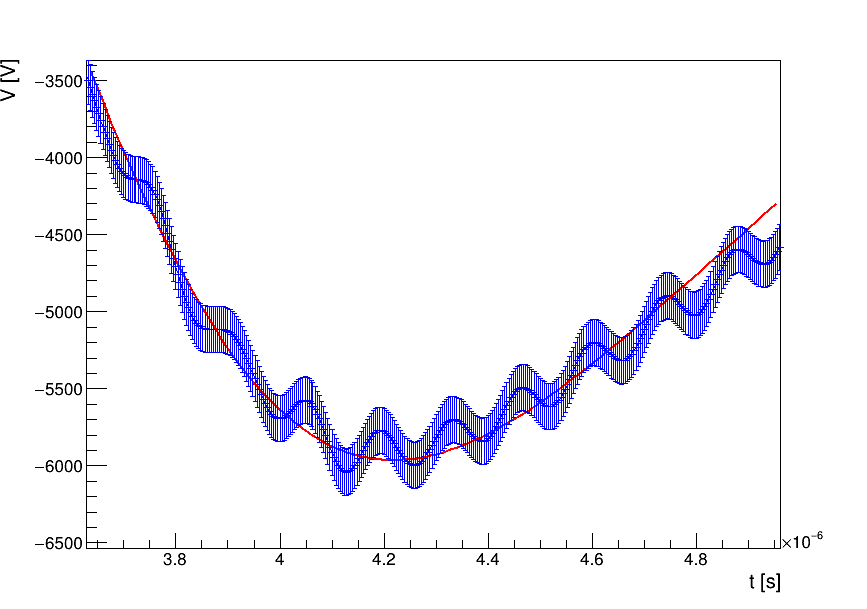
\includegraphics[width=.6\textwidth]{Immagini/esfiterr.png}
\caption{Esempio di fit del picco di tensione, $f = \SI{5}{\kilo\hertz}$ e $\Delta t = \SI{16}{\micro\second}$}
\label{fig:landau}
\end{figure}


Le tensioni del picco così calcolate, al variare della duty cycle per le diverse frequenze, sono presentate in figura \ref{fig:tensioni}.
Per tutte le frequenze di lavoro tra i $\SI{4}{\micro\second}$ e i $\SI{16}{\micro\second}$ risulta un andamento lineare, con tensione variabile tra i $\SI{2}{\kilo\volt}$ e i $\SI{9}{\kilo\volt}$. Aumentando ancora il tempo di apertura del circuito la tensione arriva a valori più elevati, fino un massimo di circa $\SI{10}{\kilo\volt}$, ma viene perso l'andamento lineare.


 \begin{figure}
\centering
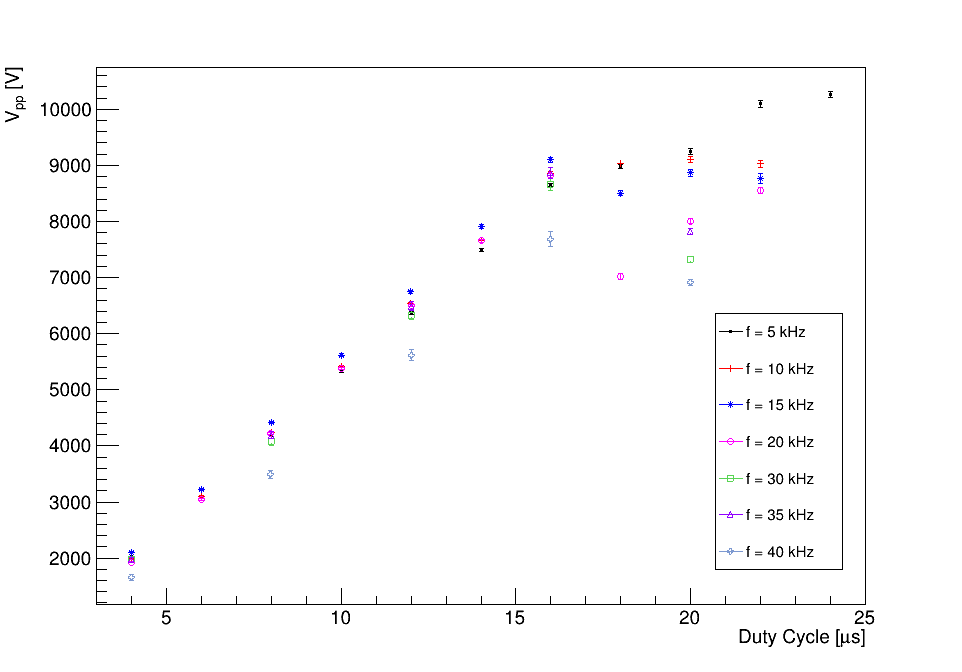
\includegraphics[width=.6\textwidth]{Immagini/nogas.png}
\caption{Tensioni al variare del tempo di apertura del circuito e per diverse frequenze.}
\label{fig:tensioni}
\end{figure}


Le misure non sembrano presentare un andamento in funzione della frequenza, per verificarlo vengono calcolati i coefficenti dell'interpolazione lineare per le varie frequenze, presentati in figura \ref{fig:fitlin}.
Viene confermata l'assenza di un andamento specifico al variare della frequenza.

\begin{figure}
\centering
\subfloat[][Pendenza delle rette.]
  {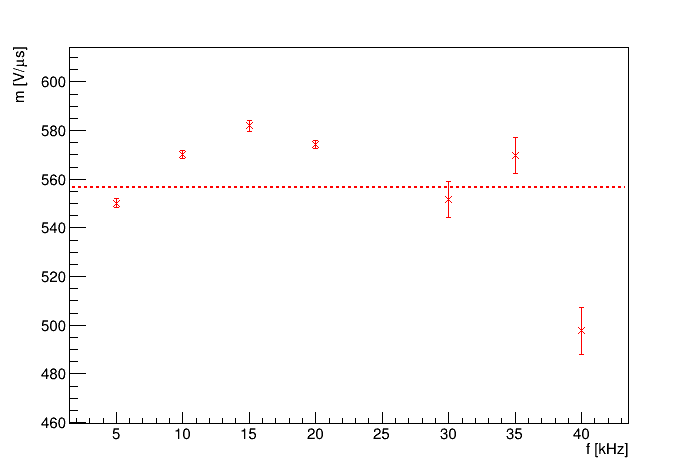
\includegraphics[width=.48\textwidth]{Immagini/m_freq_nogas.png}}
\subfloat[][Intercetta delle rette.]
  {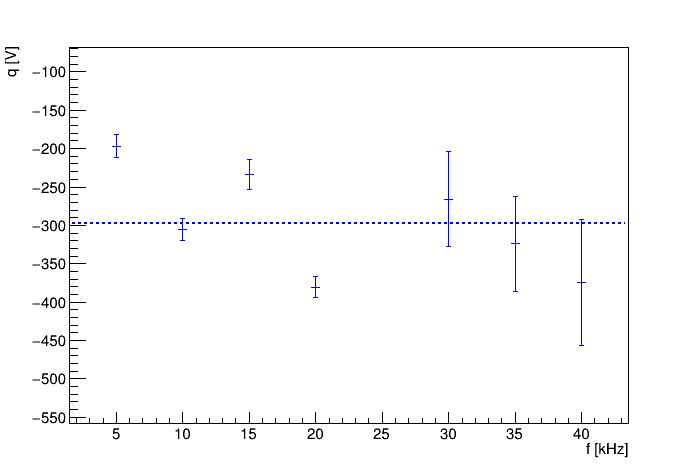
\includegraphics[width=.48\textwidth]{Immagini/q_freq_nogas.png}}
\caption{Parametri dell'interpolazione lineare dei set di misure senza immissione di gas(nel range $\Delta t$ stabilito), al variare della frequenza.}
\label{fig:fitlin}
\end{figure}

\end{comment}


\begin{comment}
\subsection{Misure con elio}
Per caratterizzare il funzionamento della sorgente nelle possibili condizioni di trattamento, vengono misurate contemporaneamente, su due diversi canali dell'oscilloscopio, tensione alla quale si trova l'elettrodo e corrente che fluisce nel plasma. Per la misura di corrente viene fatto impattare il plasma su una piastra di rame  di dimensioni \SI{2}{\centi\metre} $\times$ \SI{2}{\centi\metre} $\times$ \SI{0.5}{\centi\metre}, ad una distanza di \SI{1}{\centi\metre} dall'elettrodo della sorgente, collegata alla sonda di corrente.
Nuovamente vengono effettuate misure al variare di frequenza ($f$) e duty cycle ($\Delta t$), con le stesse modalità delle misure di tensione.
Tutte le misure sono effettuate con flusso di gas He pari a $\SI{2}{\litre/\minute}$.
Si ottengono curve come in figura \ref{fig:corrente_es}.

\begin{figure}
\centering
 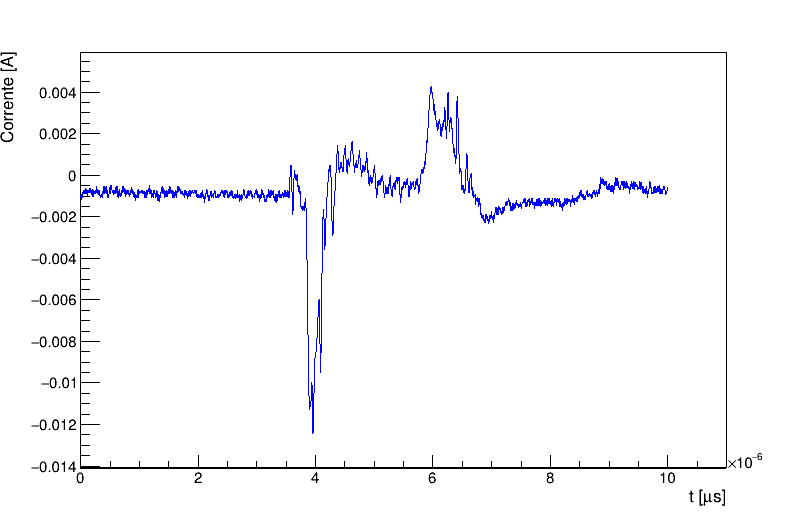
\includegraphics[width=.7\textwidth]{Immagini/corrente_es.png}
\caption{Esempio di misure di corrente per $f = \SI{5}{\kilo\hertz}$ e $\Delta t = \SI{24}{\micro\second}$, prototipo 1.}
\label{fig:corrente_es}
\end{figure}



\subsection{Tensione e corrente con elio}
Le misure di tensione presentano l'andamento trovato precedentemente, mentre le misure di corrente presentano un primo picco negativo seguito da un picco più basso di segno opposto, positivo. L'analisi proposta è uguale a quella pensata per i set di misure precedenti: vengono tagliate le oscillazioni ad alta frequenza, ricostruito il segnale (aggiungendo l'errore dovuto al taglio delle alte frequenze e agli strumenti di misura) e il valore del minimo viene trovato interpolando con una funzione di Landau. Da questo fit vengono calcolati valori e posizione del picco di tensione, del picco negativo di corrente e del picco positivo di corrente.
In figura \ref{fig:landau} un esempio del fit.

\begin{figure}
\centering
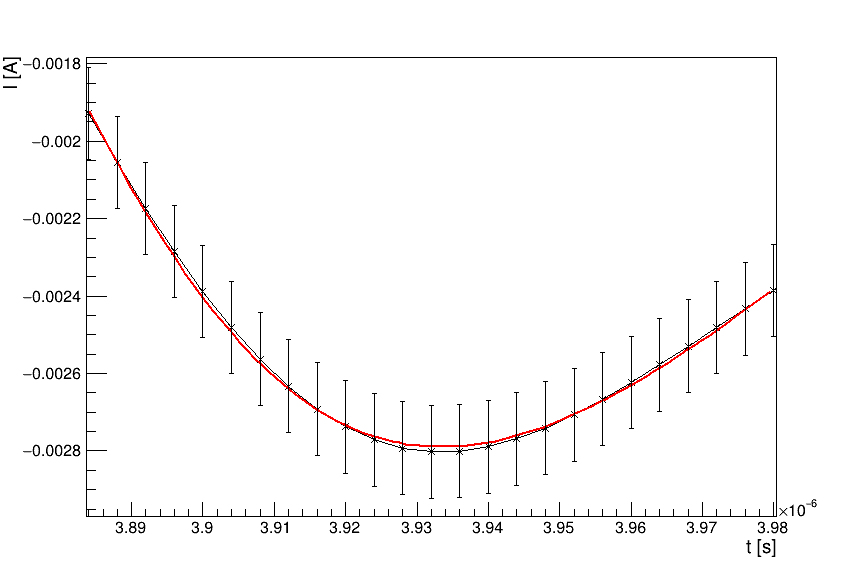
\includegraphics[width=.6\textwidth]{Immagini/es_fit_landau.png}
\caption{Esempio di fit del picco di corrente, $f = \SI{5}{\kilo\hertz}$ e $\Delta t = \SI{24}{\micro\second}$}
\label{fig:landau}
\end{figure}

Le tensioni del picco così calcolate, al variare della duty cycle per le diverse frequenze, sono presentate in figura \ref{fig:picchi}.
Nuovamente troviamo un andamento lineare per la tensione tra i $\num{4}$ e i $\SI{16}{\micro\second}$. Anche il picco negativo di corrente presenta questo andamento lineare, mentre per il picco positivo non è possibile identificare un comportamento simile, i valori si disperdono.

\begin{figure}
\centering
\subfloat[][Modulo del picco di tensione.]
  {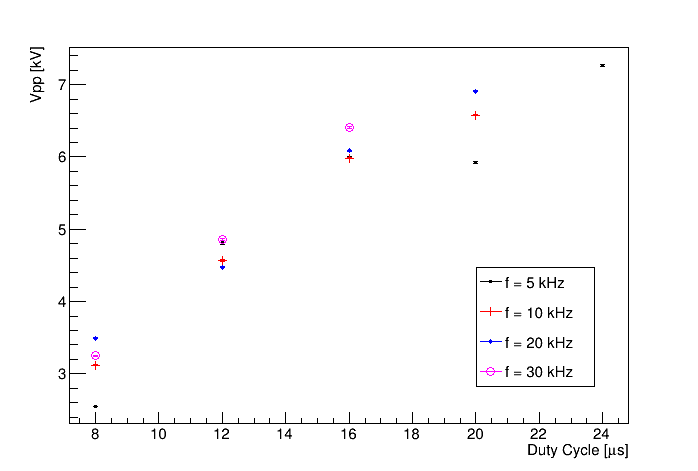
\includegraphics[width=.65\textwidth]{Immagini/vpp_corrente.png}}
\\
\subfloat[][Modulo del picco primario di corrente.]
  {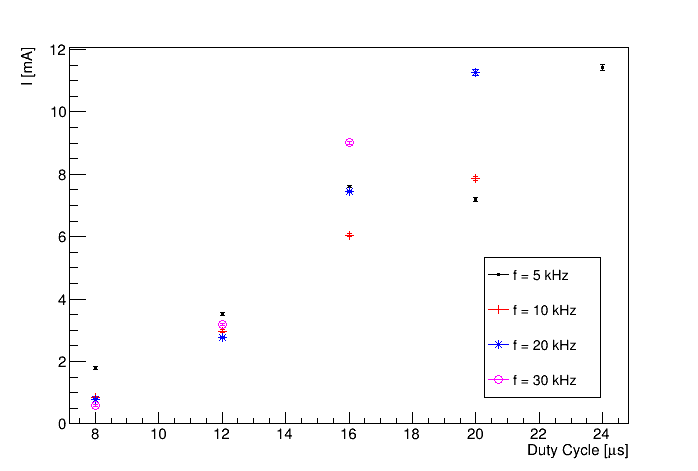
\includegraphics[width=.65\textwidth]{Immagini/I1_corrente.png}}
\\
\subfloat[][Picco secondario di corrente.]
  {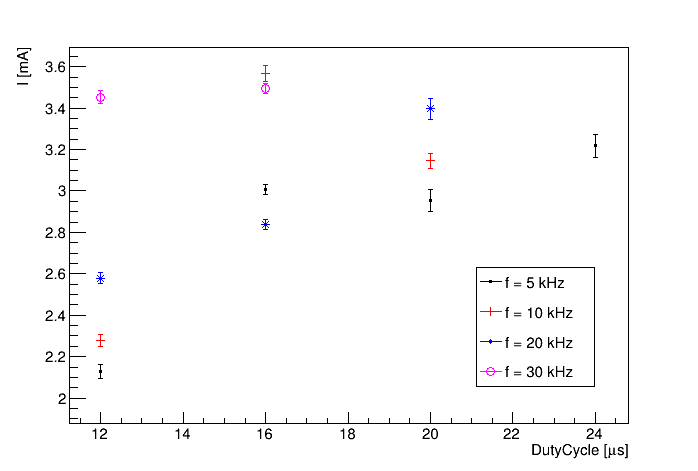
\includegraphics[width=.65\textwidth]{Immagini/I2_corrente.png}}
\caption{Valori dei picchi misurati al variare del tempo di apertura del circuito e per diverse frequenze.}
\label{fig:picchi}
\end{figure}


Nuovamente, per visualizzare in maniera esplicita l'effetto della variazione della frequenza, vengono calcolati i coefficenti dell'interpolazione lineare per le tensioni di picco e per le correnti di picco negativo, presentati in figura \ref{fig:fitlin_cor}. 
Per le tensioni risulta un comportamento identico al precedente, dove i valori si assestano attorno una media lievemente inferiore rispetto le misure in assenza di elio.
Per il valore massimo di corrente viene trovato un aumento in funzione della frequenza di funzionamento della sorgente.

\begin{figure}
\centering
\subfloat[][Pendenze dei picchi di tensione.]
  {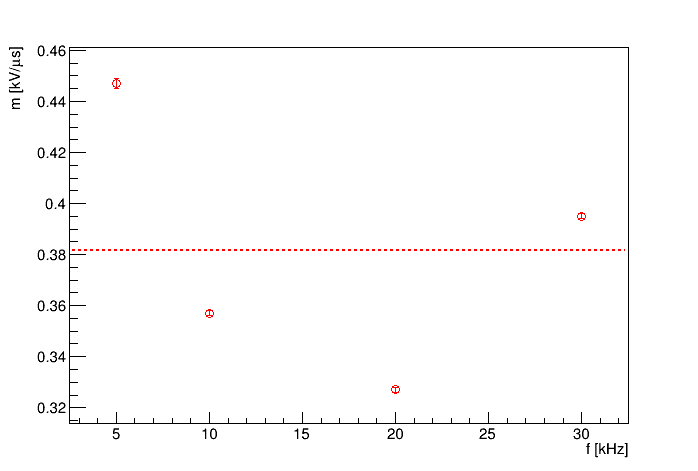
\includegraphics[width=.48\textwidth]{Immagini/mVpp_cor.png}}
\subfloat[][Intercette dei picchi di tensione.]
  {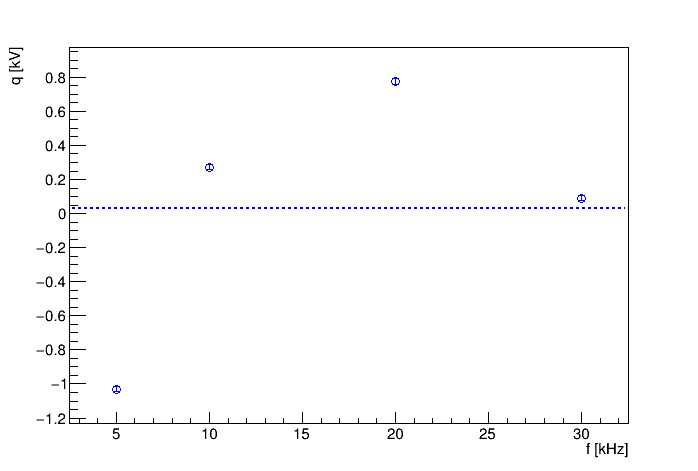
\includegraphics[width=.48\textwidth]{Immagini/qVpp_cor.png}}
\newline
\subfloat[][Pendenze dei picchi di corrente.]
  {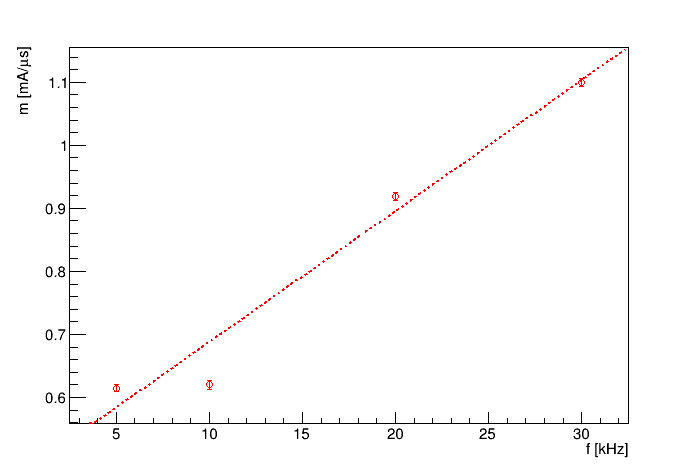
\includegraphics[width=.48\textwidth]{Immagini/mI1_cor.png}}
\subfloat[][Intercette dei picchi di corrente.]
  {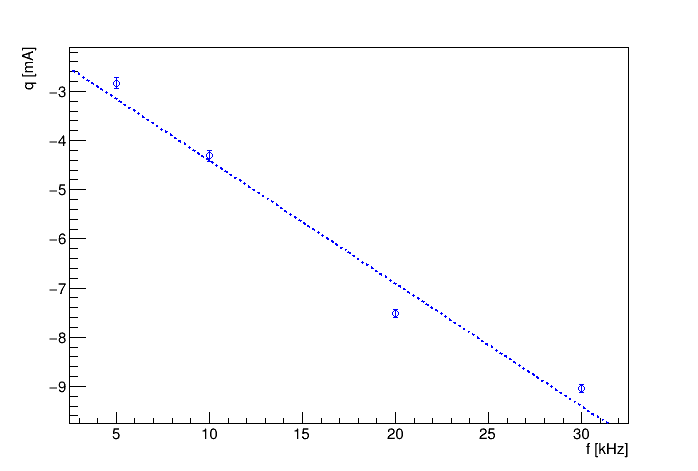
\includegraphics[width=.48\textwidth]{Immagini/qI1_cor.png}}
\caption{Parametri dell'interpolazione lineare dei picchi delle misure di tensione e corrente.}
\label{fig:fitlin_cor}
\end{figure}

\end{comment}



\begin{comment}

Data la possibilità di visualizzare contemporaneamente sia la tensione sia la corrente in uscita dal circuito, viene proposta un'analisi delle variazioni temporali tra i diversi picchi. In particolare viene calcolato il tempo tra i due picchi di corrente e tra il picco di tensione e il picco di corrente primario, mostrati in figura \ref{fig:tempi}.
In entrambi i casi non è possibile estrapolare un andamento particolare, indicando che non vi sono differenze significative nei tempi di salita dei picchi al variare del tempo di apertura del circuito e della frequenza.

\begin{figure}
\centering
\subfloat[][Tempo tra i picchi di corrente.]
  {\includegraphics[width=.48\textwidth]{Immagini/ti2ti1.png}}
\subfloat[][Tempo tra picco tensione e primo picco di corrente.]
  {\includegraphics[width=.48\textwidth]{Immagini/ti1tv.png}}
\caption{Misura delle differenze temporali tra i picchi.}
\label{fig:tempi}
\end{figure}

\end{comment}
